\documentclass{beamer}
\usetheme{Boadilla}
\usepackage[thinc]{esdiff}
\usepackage{siunitx}
\usepackage{booktabs}
\usepackage{xcolor}
\usepackage{transparent}
\usepackage{graphicx}
\usepackage{subcaption}
\usepackage{tikz}
\usepackage[x11names]{xcolor}

\setbeamertemplate{bibliography item}[text]
\bibliographystyle{apalike}
\newcommand{\backupbegin}{
   \newcounter{finalframe}
   \setcounter{finalframe}{\value{framenumber}}
}
\newcommand{\backupend}{
   \setcounter{framenumber}{\value{finalframe}}
}


\setbeamertemplate{frametitle}[default][center]

\subtitle{}
\title{}
%\titlegraphic{\includegraphics[width=0.9\linewidth,height=0.4\linewidth]{image.png}}
\author{Ole Merkes}
\institute{University of Hamburg}
\date{\today}


\AtBeginSection[]
{
    \begin{frame}
        %\frametitle{Table of Contents}
        \tableofcontents[currentsection,currentsubsection]
    \end{frame}
}

\begin{document}

% \setbeamertemplate{background canvas}{
% \transparent{0.4}\includegraphics[width=\paperwidth,height=\paperheight]{image.png}
% }%
\begin{frame}
    \titlepage
\end{frame}
%\setbeamertemplate{background canvas}[default]


% \begin{frame}
%     \frametitle{Scaling of the HC}
%     \begin{block}{Angular momentum conserving}  
%     \begin{align}
%         \Phi_H\sim&\left(\frac{gH\Delta_h}{\Omega^2R_E^2}\right)^{1/2}\\
%         \psi_\mathrm{max} \sim & \frac{1}{\tau}\frac{g^{3/2}(H\Delta_h)^{5/2}}{\Omega^3R_E^2\Delta_v}
%     \end{align}
%     \end{block}
%     \begin{block}{Baroclinic instability and eddy flux}
%         \begin{align}
%             \theta_C \sim& \left(\frac{NH}{2\Omega a}\right)^{1/2}\\
%             \psi(1-Ro)\approx& \frac{S}{f}
%         \end{align}
%     \end{block}
% \end{frame}

\begin{frame}
    \frametitle{ECHAM mean meridional circulation}
    \begin{figure}
        \centering
        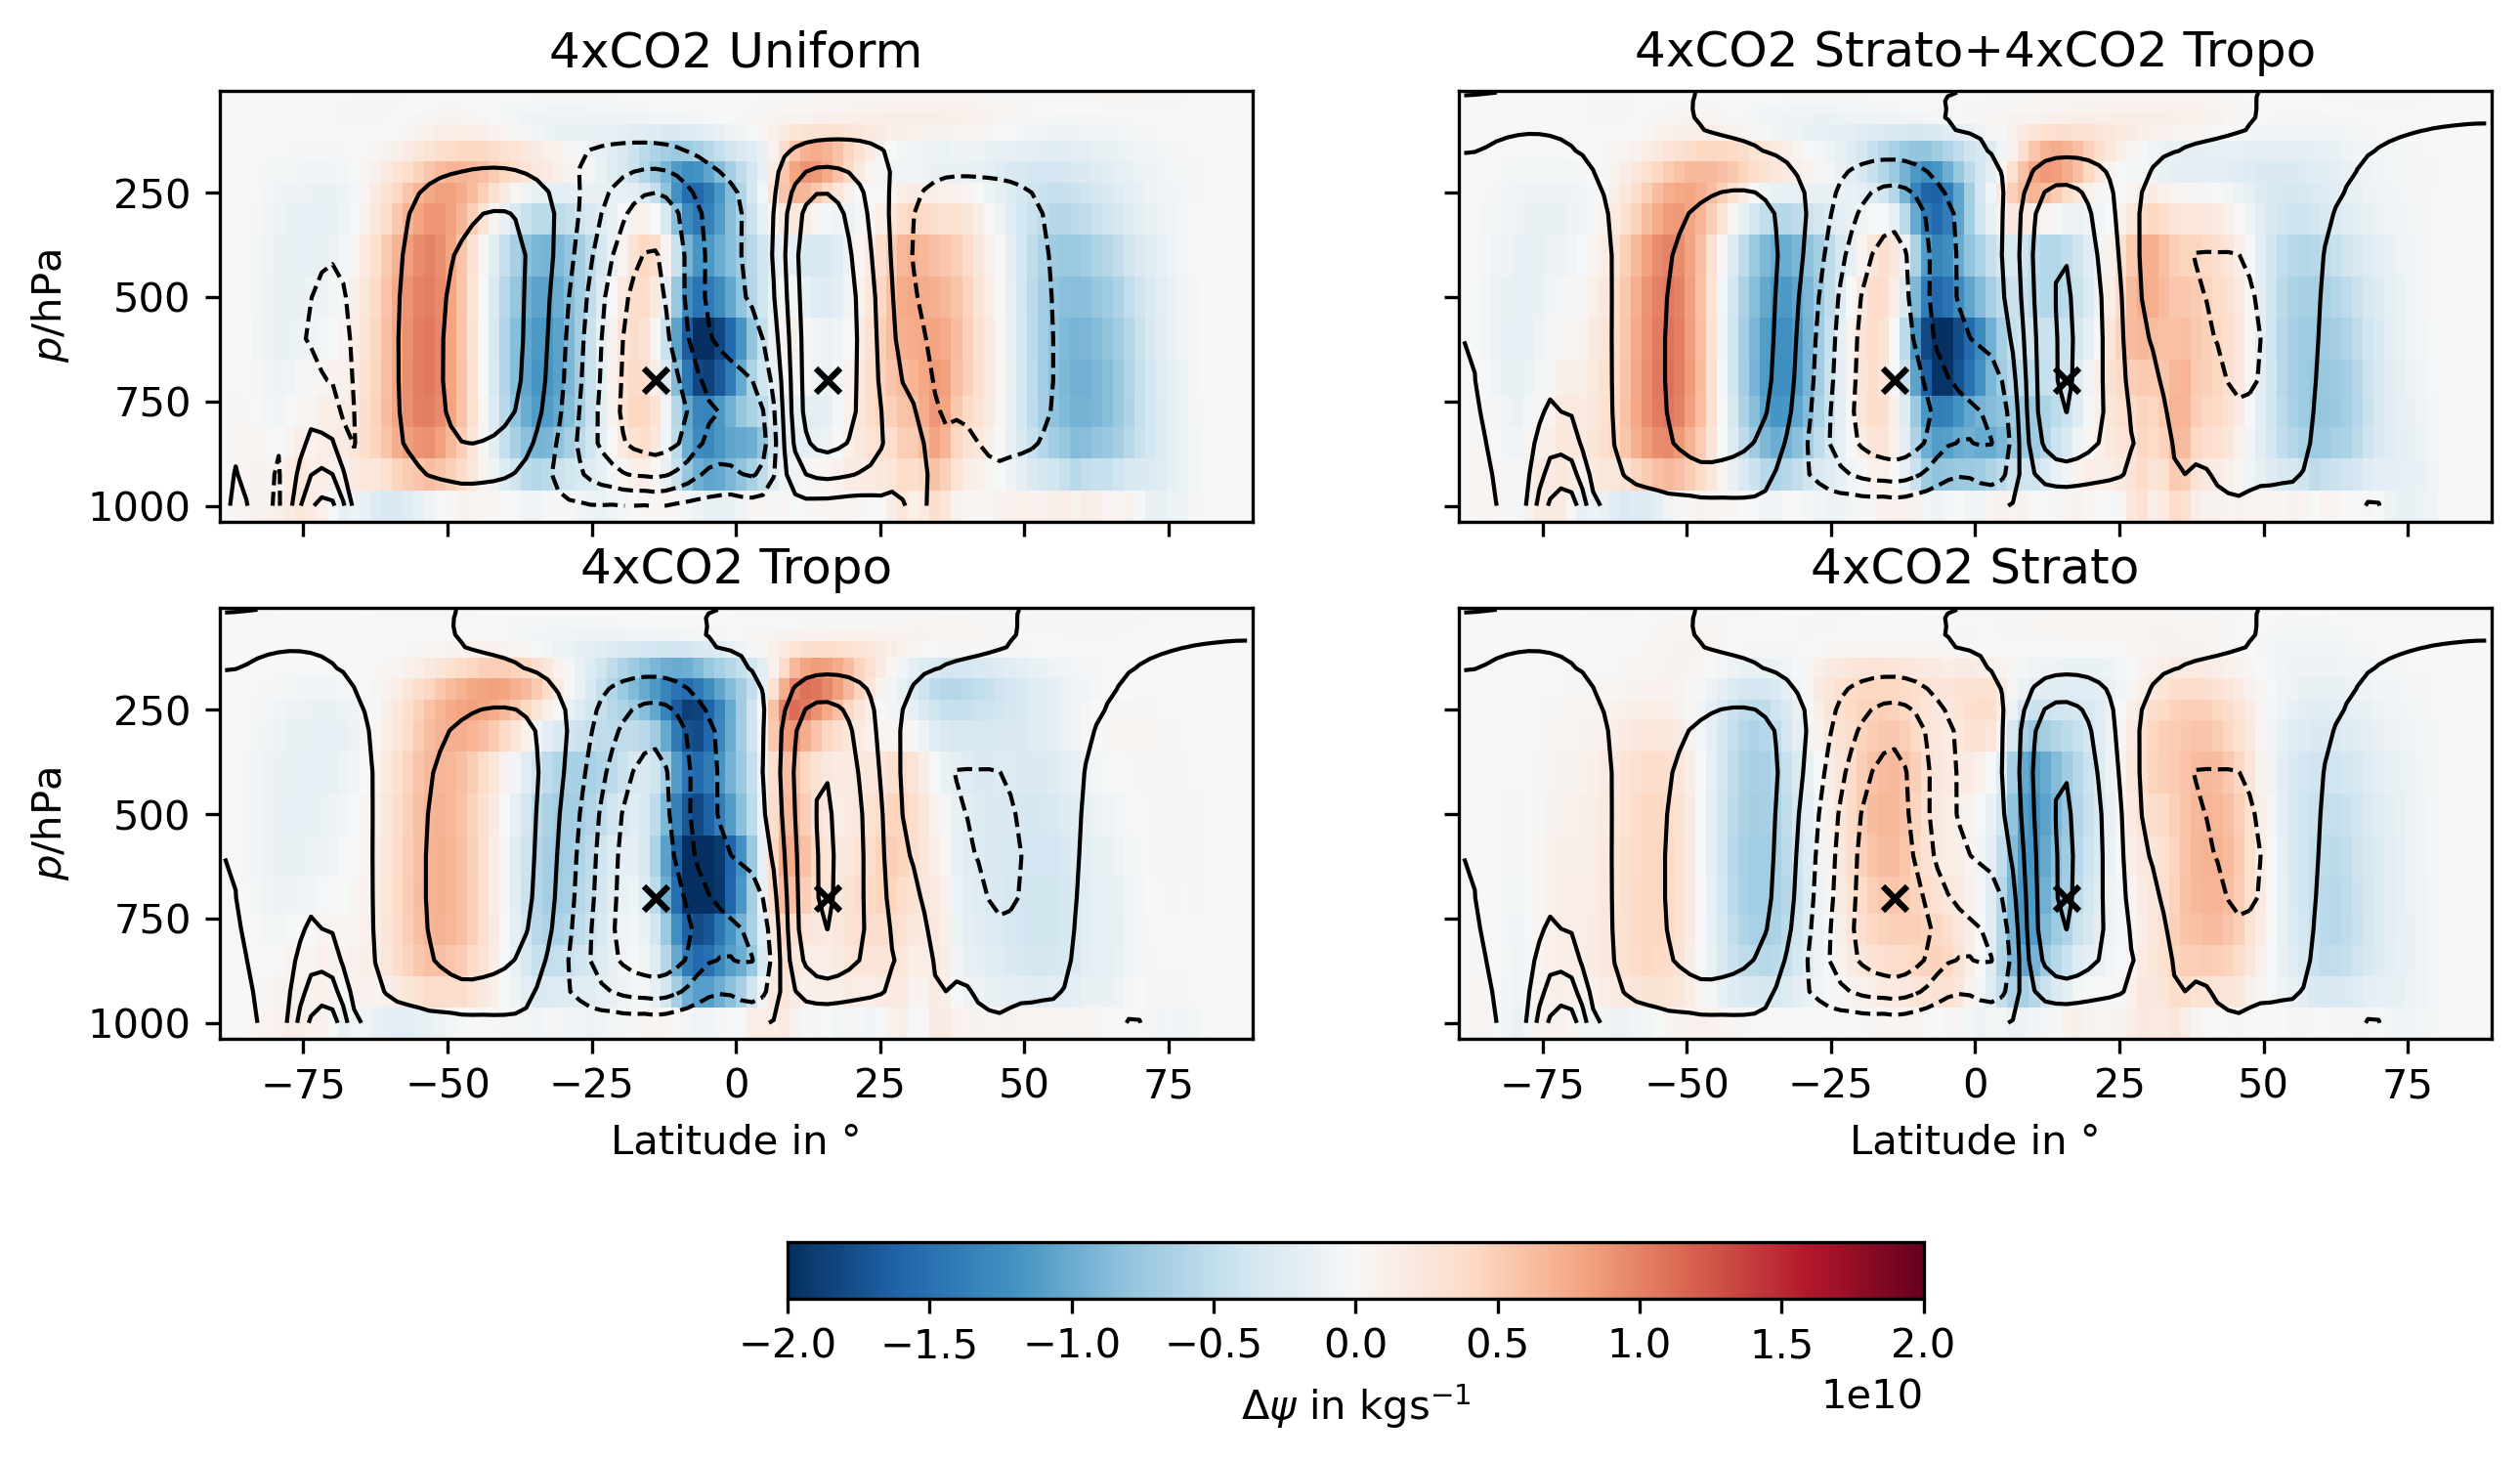
\includegraphics[width=\textwidth]{figures/HC.png}
    \end{figure}
\end{frame}


\begin{frame}
  \frametitle{Changes in Hadley circulation}
\begin{table}[]
    \centering
    \begin{tabular}{cc|ccc}
        & PI Control &Uniform & Tropo & Strato \\ \toprule
        $\psi_\mathrm{max, NH}$& $7.72\cdot10^{10}\;\unit{\kg\s^{-1}}$ & $-1.6\%$ & $3.3\%$& $-8.7\%$\\
        $\psi_\mathrm{max, SH}$&$-9.64\cdot10^{10}\;\unit{\kg\s^{-1}}$ & $-1.4\%$ & $5.6\%$ & $-5.7\%$\\ 
        $\Phi_\mathrm{H, NH}$ & $29.2\unit{\degree}$ & $1.6\unit{\degree}$& $0.76\unit{\degree}$ &$0.76\unit{\degree}$\\
        $\Phi_\mathrm{H, SH}$ &$-30.4\unit{\degree}$ & $-1.6\unit{\degree}$& $-1.0\unit{\degree}$ &$-0.6\unit{\degree}$\\
    \end{tabular}
    \label{tab:placeholder}
\end{table}
\end{frame}

\begin{frame}
    \frametitle{Linearisation of H\&H scaling}
    \begin{block}{H\&H}  
    \begin{align}
        \Phi_H\sim&\left(\frac{gH\Delta_h}{\Omega^2R_E^2}\right)^{1/2}\\
        \psi_\mathrm{max} \sim & \frac{1}{\tau}\frac{g^{3/2}(H\Delta_h)^{5/2}}{\Omega^3R_E^2\Delta_v}
    \end{align}
    \end{block}
    \begin{block}{Linearisation}
        \begin{align}
            \frac{\delta\Phi_H}{\Phi_H} = \frac{1}{2}\frac{\delta H}{H}+\frac{1}{2}\frac{\delta\Delta_h}{\Delta_h}\\
            \frac{\delta\psi}{\psi} = \frac{5}{2}\frac{\delta H}{H}+\frac{5}{2}\frac{\delta\Delta_h}{\Delta_h}-\frac{\delta\Delta_v}{\Delta_v}
        \end{align}
    \end{block}
\end{frame}

\begin{frame}
    \frametitle{Scatter anomalies NH}
    \begin{figure}
        \centering
        
\includegraphics[width=\textwidth]{figures/scatter_NH.png}
    \end{figure}
\end{frame}

\begin{frame}
    \frametitle{Scatter anomalies SH}
    \begin{figure}
        \centering
        
\includegraphics[width=\textwidth]{figures/scatter_SH.png}
    \end{figure}
\end{frame}

\begin{frame}
    \frametitle{Applying H\&H linearisation NH}
    \begin{figure}
        \centering
        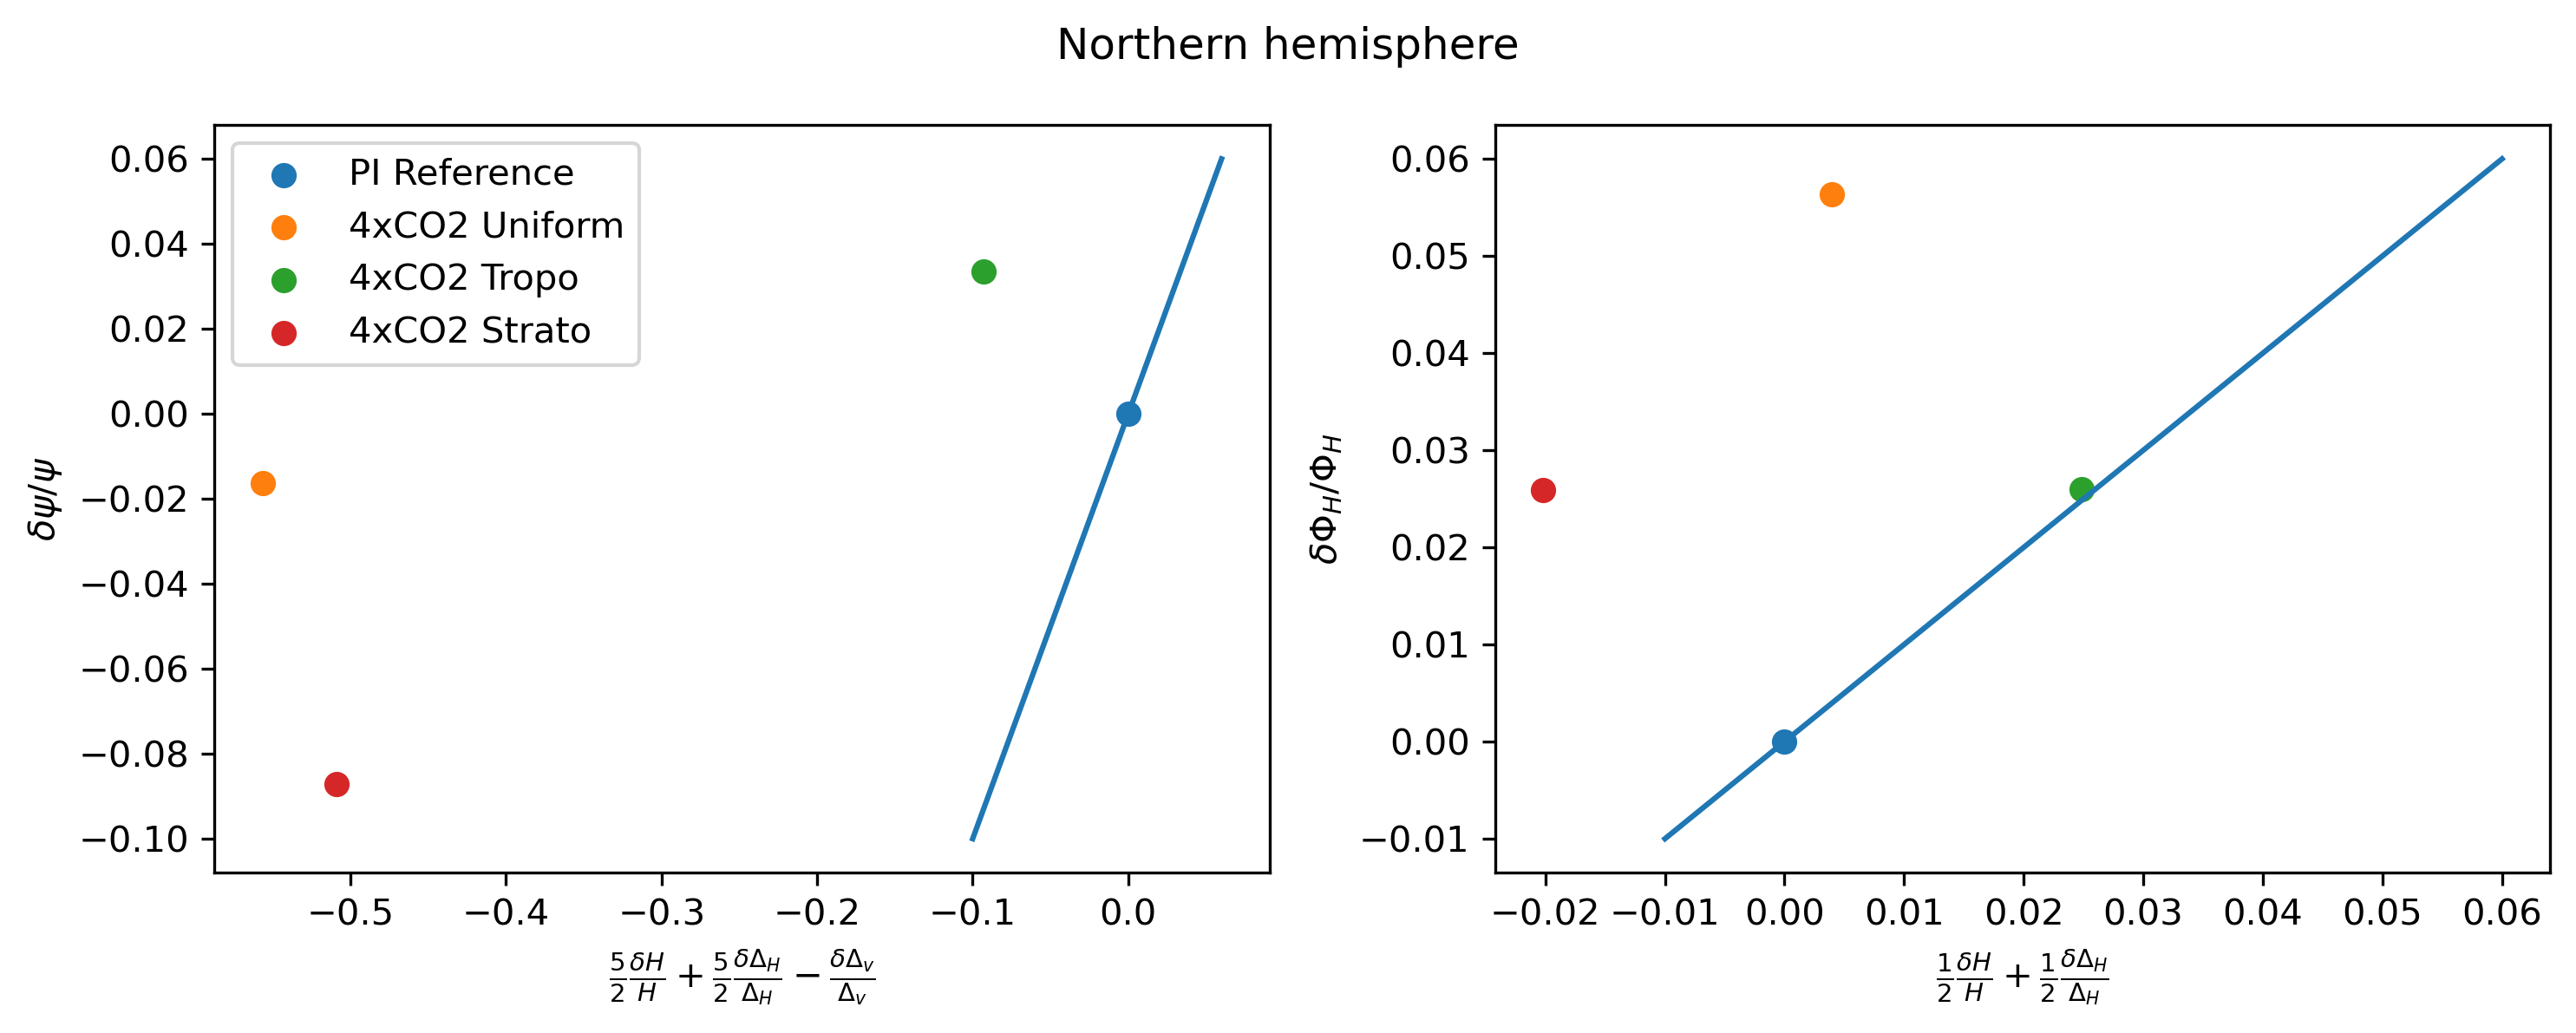
\includegraphics[width=\textwidth]{figures/HH_linear_NH.png}
    \end{figure}
\end{frame}

\begin{frame}
    \frametitle{Applying H\&H linearisation SH}
    \begin{figure}
        \centering
        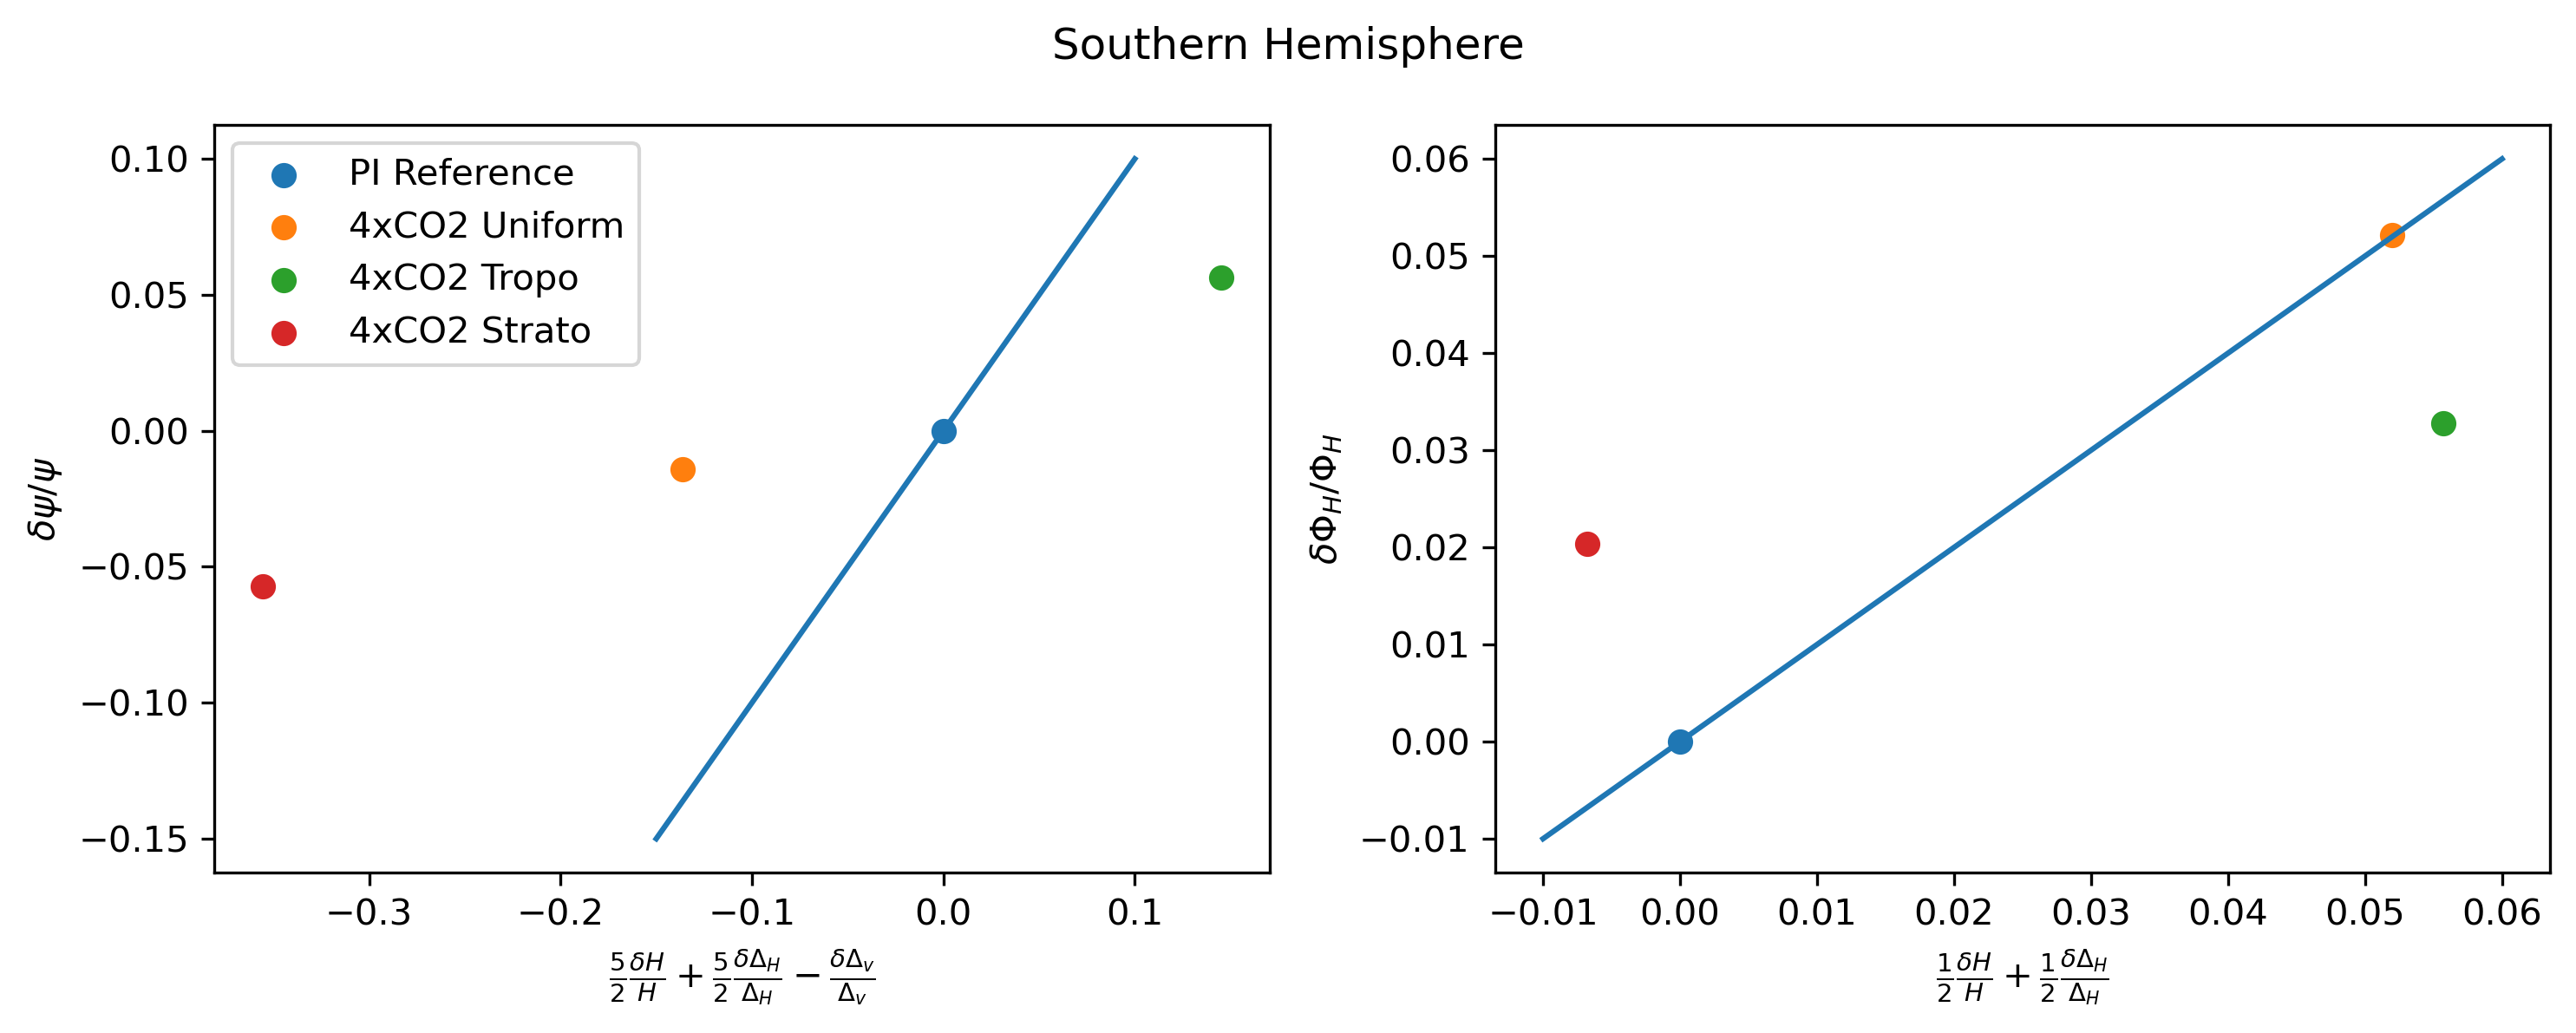
\includegraphics[width=\textwidth]{figures/HH_linear_SH.png}
    \end{figure}
\end{frame}

\begin{frame}
    \frametitle{Temperature anomalies}
    \begin{figure}
        \centering
        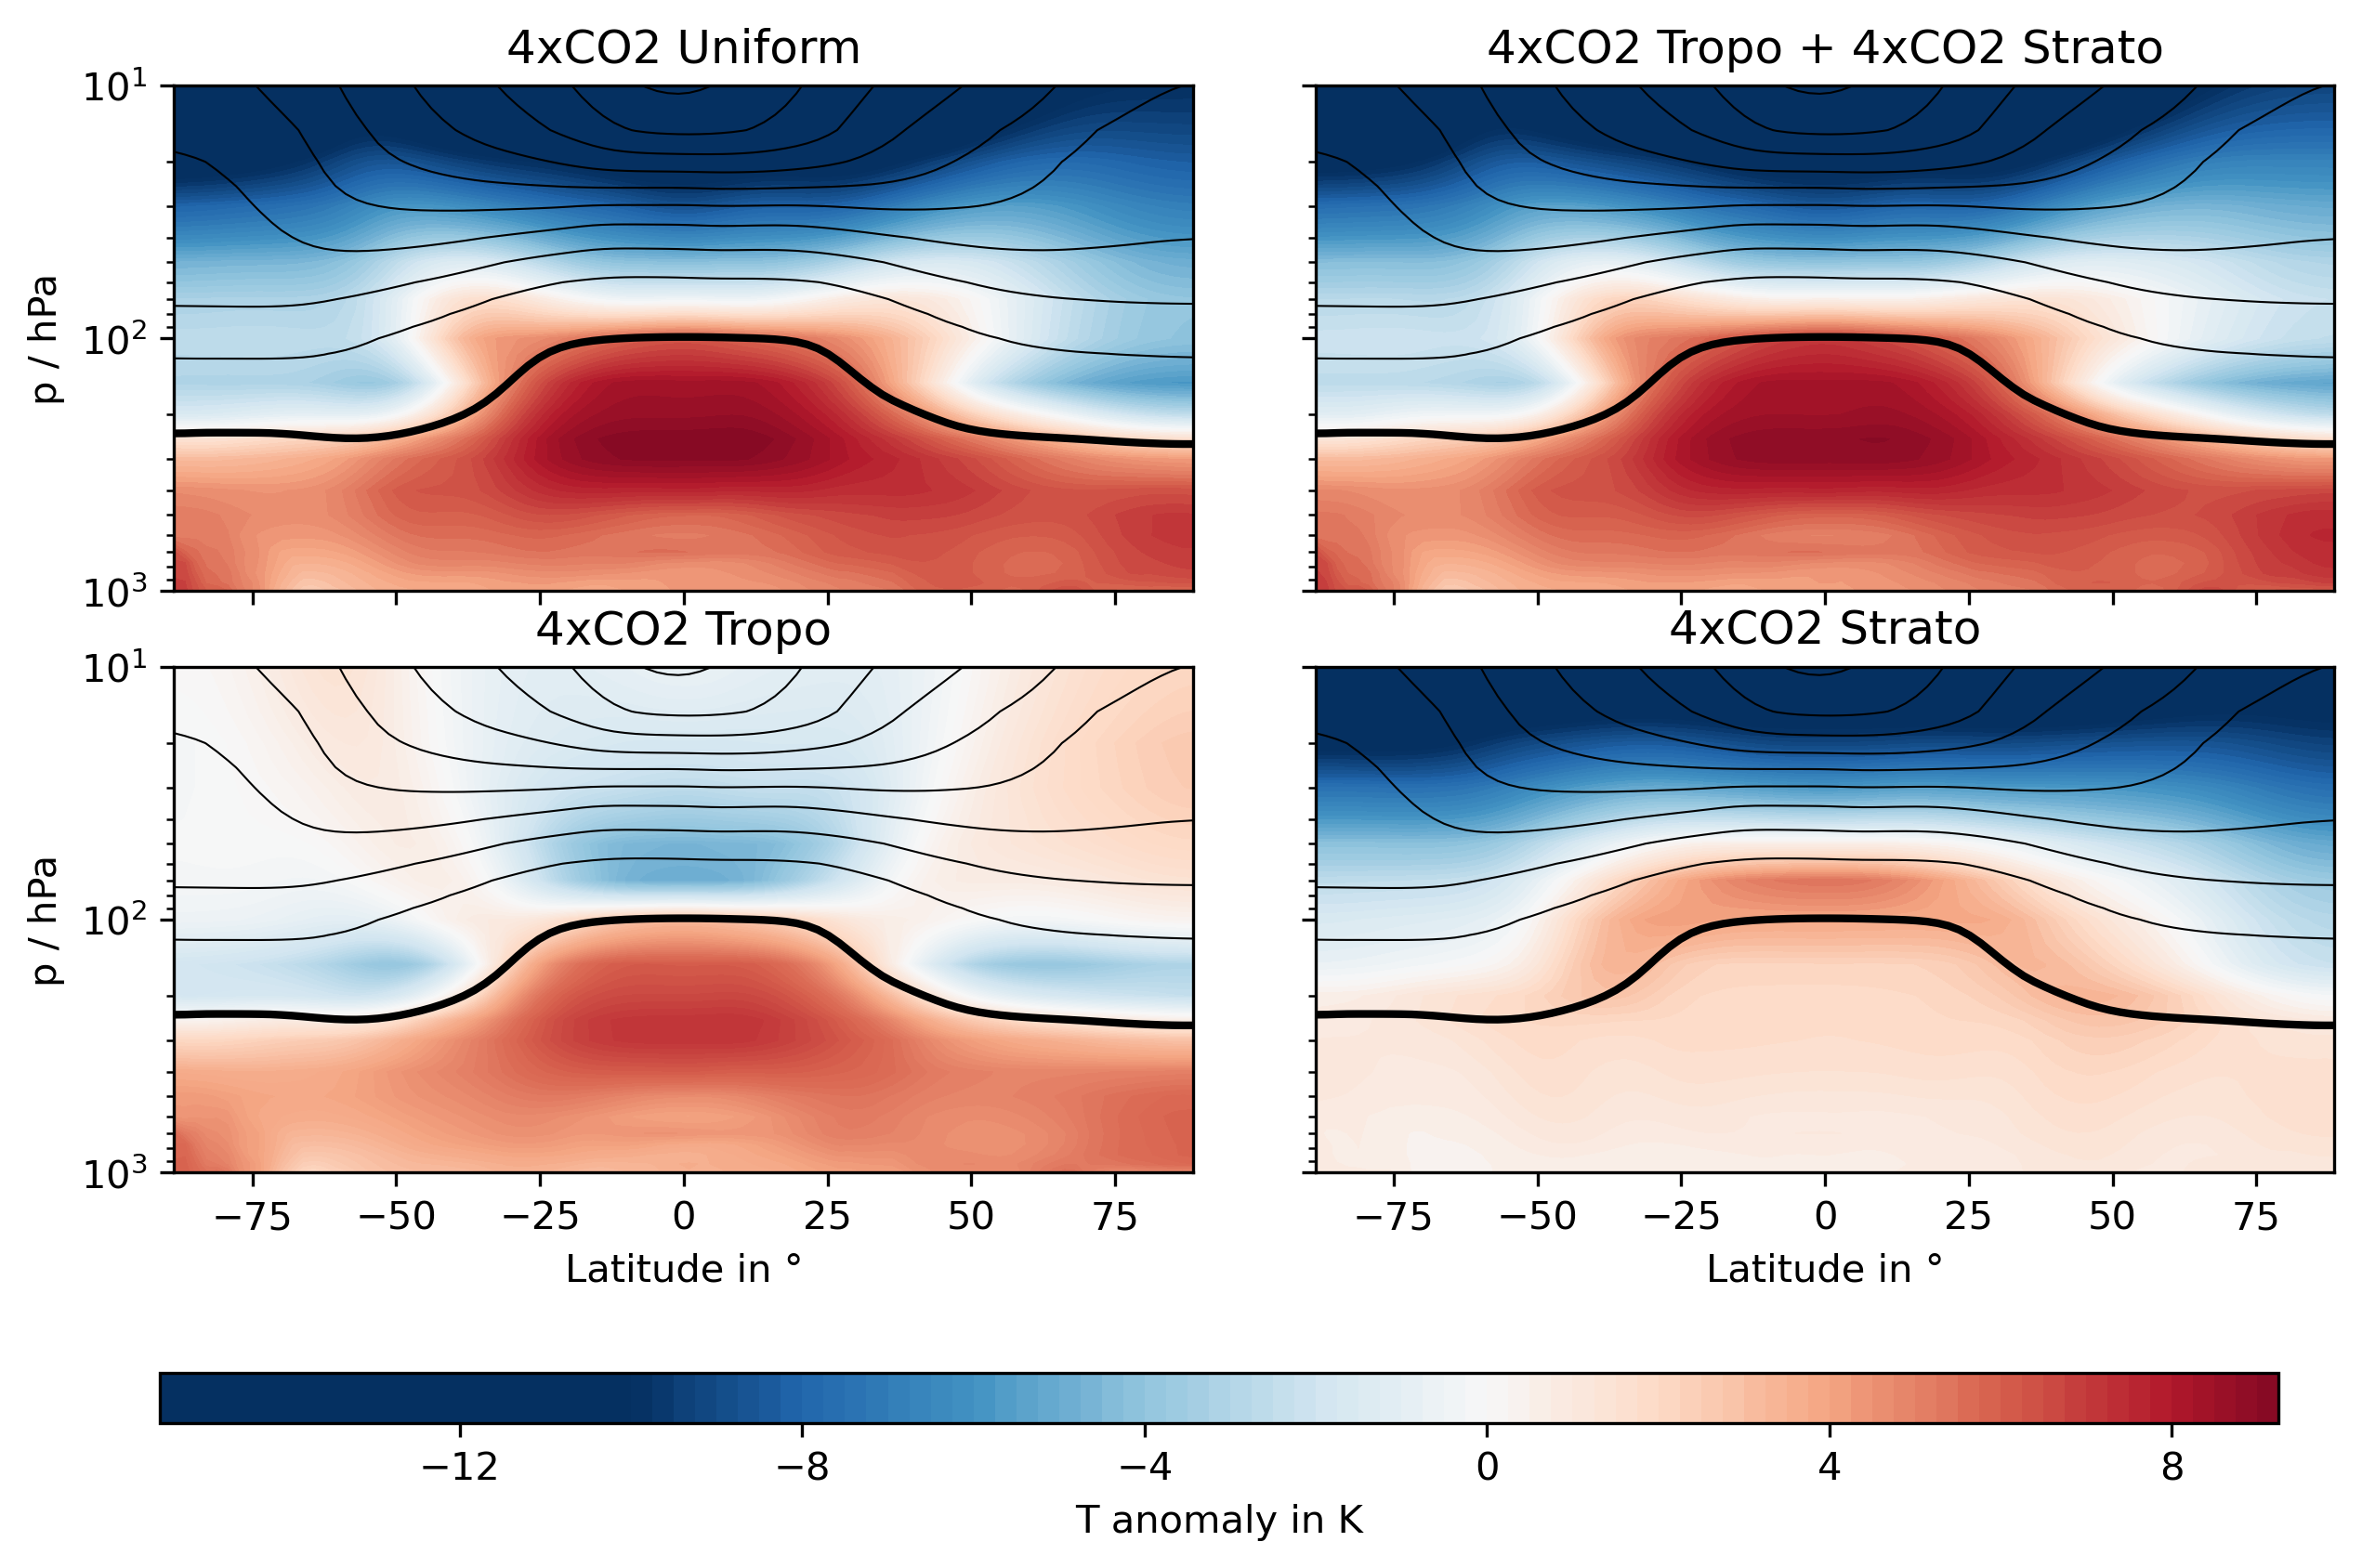
\includegraphics[width=\textwidth]{figures/T_anomalies.png}
    \end{figure}
\end{frame}

\begin{frame}
    \frametitle{1D-RE simulation from Rodrigo Caballero}
    \begin{figure}
        \centering
        \includegraphics[width=\textwidth]{../../figures/linepyline_rodrigo/trop_strat_co2.pdf}
    \end{figure}
    \begin{block}{Heating rate}
        \begin{equation}
            Q\sim\frac{\partial \tau}{\partial z}
        \end{equation}
    \end{block}
\end{frame}

\begin{frame}
    \centering
    Backup
\end{frame}



\backupbegin

\begin{frame}
    \frametitle{Definitions D'Agostino et al. 2017}
    \begin{itemize}
        \item meridional near-surface(averaged between the 700 and 800 hPa levels) potential
        temperature contrast $\Delta_h\theta(p,\varphi)=\Bar{\theta}(800-700\;\si{hPa},0-10\;\unit{\degree})-\Bar{\theta}(800-700\;\si{hPa},40-60\;\si{\degree})$
        \item subtropical near-surface static stability $\Delta_v\theta(p,\varphi)=\Bar{\theta}(\textcolor{red}{200}\;\si{hPa},20-40\;\unit{\degree})-\Bar{\theta}(800\;\si{hPa},20-40\;\si{\degree})$
        \item tropical tropopause pressure height $p_t(\varphi)=\Bar{p}(15\unit{\degree S}- 15\unit{\degree N})$ 
        \item extratropical tropopause height $p_{et}(\varphi)=\Bar{p}(35\unit{\degree}- 55\unit{\degree})$ (Lu et al. 2007)
    \end{itemize}
\end{frame}
\backupend
\end{document}
